\documentclass[12pt,twoside]{article}
\usepackage{jmlda}

\makeatletter
\bibliographystyle{unsrt}
\renewcommand{\@biblabel}[1]{#1.}
\makeatother

%\NOREVIEWERNOTES
\title
    [Аппроксимация фазовой траектории] 
    % Краткое название; не нужно, если полное название влезает в~колонтитул
    {Аппроксимация фазовых траекторий квазипериодических временных сигналов с помощью сферических гармоник}
\author
    {Тихонов~Д.\,М., Стрижов~В.\,В.} % основной список авторов, выводимый в оглавление
    %\thanks
    %{Работа выполнена при финансовой поддержке РФФИ, проект \No\,00-00-00000.}
%\email
   % {author@site.ru}
%\organization
   % {$^1$Организация; $^2$Организация}
%\thanks
%	{ }
\abstract
{\textbf{Аннотация}: В этой работе обсуждается проблема построения модели аппроксимации квазипериодических сигналов наименьшей структурной сложности.
Для этого с помощью метода задержек производится переход в фазовое пространство.
Для упрощения модели в фазовом пространстве выбирается подпространство.
Вводится критерий выбора размерности подпространства.
Фазовая траектория в полученном подпространстве аппроксимируется с помощью сферических гармоник.
Эксперимент проведен на показателях акселерометра мобильного устройства с различными классами движений человека.

\bigskip
\textbf{Ключевые слова}: \emph {временные ряды, аппроксимация, фазовое пространство, сферические гармоники}.}

    

\newcommand{\nsymbol}[2]{\medskip\hangindent=\parindent\hangafter=1\noindent $#1$ --- #2\par}
\newcommand{\nsymbolp}[3]{\nsymbol{#1}{#2 \dotfill\pageref{#3}}}

\newcommand{\hookuparrow}{\mathrel{\rotatebox[origin=t]{270}{$\hookleftarrow$}}}
\newcommand{\hookdownarrow}{\mathrel{\rotatebox[origin=t]{90}{$\hookleftarrow$}}}
\begin{document}
\maketitle

\section{Введение}
Работа посвящена аппроксимации квазипериодических временных рядов.
Примерами таких рядов являются показатели акселерометра и гироскопа во время повторяющейся физической активности, электрокардиограмма и тд [...].

Различные другие методы аппроксимации имеют свои ограничениями и недостатками.
Во-первых, большинство доступных результатов предлагают решения проблемы на плоскости, т. Е. Только с данными размерности два, см., Например, [8], [9] и ссылки в них (см. Также [14] для обсуждения трехмерный [3-D] случай). Во-вторых, большинство существующих методов основано на минимизации критериев «алгебраического расстояния» (или ошибки уравнения) [2], [8], [22]. Эти критерии могут не иметь четкой геометрической интерпретации, поскольку они не связаны напрямую с геометрическими евклидовыми расстояниями от точек до кривой, как это подробно обсуждается в [9]. В-третьих, большинство доступных результатов (за исключением работы в [8], для которой, однако, верны два предыдущих пункта) основаны на итеративных схемах нелинейной оптимизации, таких как модификации алгоритма Гаусса-Ньютона,
	
Для аппроксимации временного ряда строится пространство фазовых траекторий.
Построения осуществляется с помощью множества векторов задержек или метод задержек.
Этот метод используется при анализе нестационарных временных рядов.
Например, в методе сингулярного спектрального анализа (singular spectrum analysis, SSA ~\cite{Golyandina2002}) разложения на компоненты и прогноз основаны на траекторной матрице.
Она позволяет перейти от одномерного (скалярного) временного ряда к многомерному (векторному) представлению.
Метод задержек так же получили широкое распространение в анализе нелинейных динамических систем~\cite{Takens1981} и т.п.

Размерность траекторного пространства оказывается избыточной ~\cite{Golyandina2002}.
Это приводит к неустойчивости исследуемых моделей и сложному описанию временного ряда.
Для понижения размерности фазового пространства предлагается использовать  метод главных компонент (PCA).
	
В выбранном пространстве уменьшенной размерности предлагается спроецировать имеющуюся траекторию на $p$-мерную единичную сферу и перейти в $p-1$-мерное сферическое пространство.
Полученную определенную на поверхности сферы функцию предлагается представить в виде ряда разложенного по сферическим функциям.

\begin{figure}[h]
\centering
  \subfloat[$s(t) = 2cos(2\pi\nu_1t + \varphi_1) + cos(2\pi\nu_2t + \varphi_2) + \varepsilon$]
  {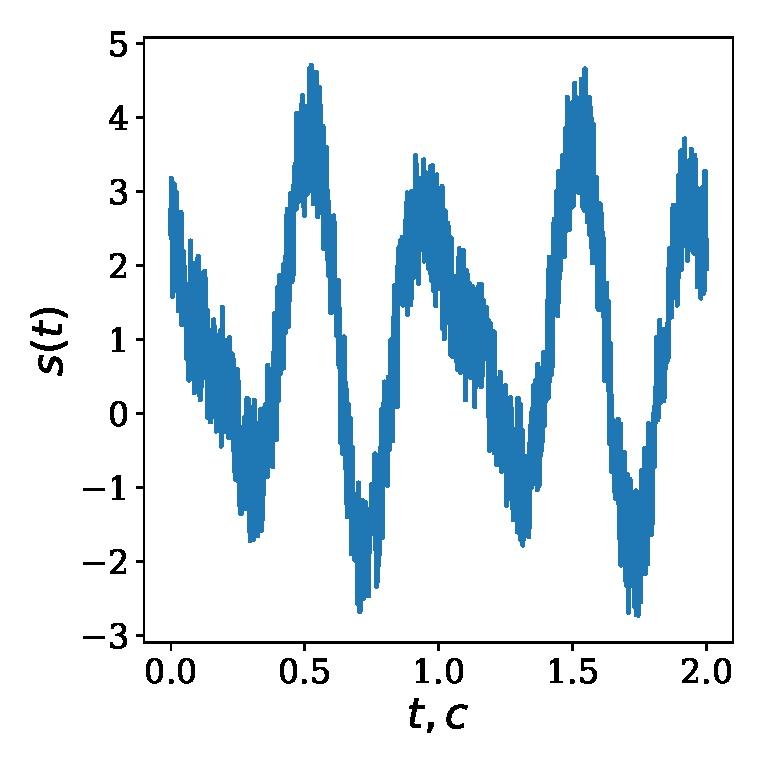
\includegraphics[width=0.25\textwidth]{figs/synthetic_example.eps}}
  \subfloat[Фазовая траеткория (PCA)]
  {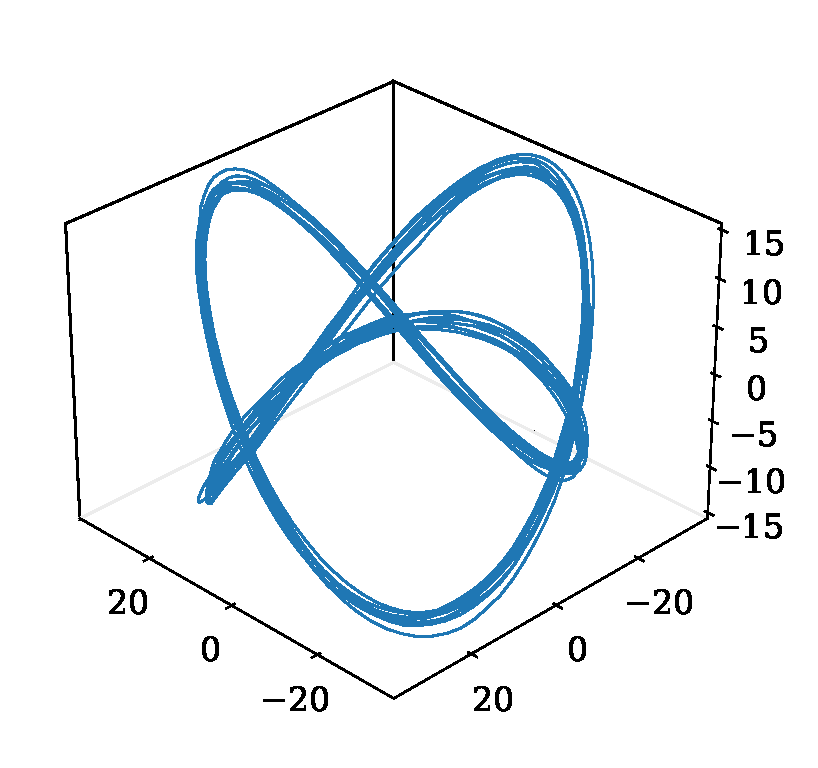
\includegraphics[width=0.3\textwidth]{figs/synthetic_trajectory.eps}}\\
\caption{Временной ряд с параметрами $\nu_1 = 2\;[\frac{1}{c}], \varphi_1 = 0,\nu_2 = 3\;[\frac{1}{c}],\varphi_2 = \frac{3\pi}{4}$ и его фазовая траетория. }
\label{fg:initial_traj}
\end{figure}

На рис.~\ref{fg:initial_traj} показан изначальный временной ряд и его разложение, пунктирной и сплошной линией соответственно, а также его фазовая траектория уменьшенная в пространство размерности 3 с помощью метода главных компонент (principal component analysis, PCA).

\section{Постановка задачи}
По имеющемуся временному ряду $\mathbf{s}=[s_1,...,s_N]^{\mathsf{T}}$ строится траекторная матрица или матрица Ганкеля

\begin{equation}
\mathbf{H_{s}} = 
\begin{bmatrix} 
	s_{1} & s_{2} & \ldots &s_{n-1} &s_{n}\\
	s_{2} & s_{3} & \ldots &s_{n} &s_{n+1}\\
	\vdots& \vdots & \ddots & \vdots & \vdots\\
	s_{N-n+1} & s_{N-n+2} &\ldots&s_{N-1} &s_{N}\\
\end{bmatrix}
\label{eq:hankel_matrix}
\end{equation}
                   
где $N$-длинна временного ряда, $n$-ширина окна, не меньшая, чем предполагаемый период. Обозначим $t$-ую строку матрицы Ганкеля $\mathbf{H_{s}}$ за $\mathbf{x_{t}}$. Матрица $\mathbf{H_{s}}$ пребразуется к:	
\begin{equation}
	\mathbf{H_{s}} = 
	\begin{bmatrix} 
                  	\mathbf{x_{1}}\\ \mathbf{x_{2}}\\
                  	\vdots\\
                  	\mathbf{x_{m}}\\
                   \end{bmatrix},
                   \mathbf{x_t}=[s_{t},s_{t+1},\ldots,s_{t+n-1}] ,
                   m = N-n+1
\label{eq:hankel_matrix_2}
\end{equation}
\vspace{\baselineskip}

Все векторы $\mathbf{x_{t}}$ принадлежат $\mathbb{H}_{\mathbf{x}} \subseteq \mathbb{R}^{n}$. Предполагается, что размерность траекторного пространства избыточна, поэтому предлагается исследовать некоторые проекции на траекторное подпространство.
Однако заранее неизвестно, в каком пространстве необходимо уменьшать размерность, поэтому задача приобретает следующий состоящий из двух вариантов вид:

\begin{equation}
	t \mapsto \mathbf{x} \mapsto \mathbb{H}_{x}^{n} \xrightarrow{} \mathbb{H}_{x}^{p} \xrightarrow{} \mathbb{S}_z^{(p)} \hookrightarrow [0,2\pi] \xrightarrow{f} r
\label{eq:goal}
\end{equation}

\vspace{\baselineskip}

\begin{Def}
Параметрическая аппроксимирующая модель временного ряда  $\mathbf{x}$  - это такое отображение $g$, что:
\begin{equation}
	g: \mathbb{R}^{q} \times \mathbf{S} \xrightarrow{} \mathbf{S}
\label{eq:param_model}
\end{equation}
\end{Def}

Предполагается, что аппроксимирующая модель строится в пространстве меньшей размерности $(p-1)$, в котором выбранное отображение $h: \mathbf{H}_{x}^{n} \xrightarrow{} \mathbf{S}_x^{(p-1)} $, где $(p-1)\ll n$, сохраняет геометрическую структуру множество точек $\mathbf{H}_{x}^{n}$. 

\begin{Def}
Структурная сложность - это количество параметров $q$ модели, позволяющих строить адекватную аппроксимацию.
\end{Def}



\section{Модели аппроксимации}
\paragraph{GAN для фазовых траекторий в 2D}

\begin{itemize}
\item \textbf{Модель генератор реальных данных}
\begin{equation}
	t \xrightarrow{} s\xrightarrow{Hankel}  \mathbf{x}_i \xrightarrow{PCA} x_i,
	\label{eq:GAN_real}
\end{equation}
где $x_i$ - точка фазовой траектории в уменьшенном пространстве, $x_i \in \mathbb{R}^2$.
\end{itemize}

\begin{itemize}
\item \textbf{Модель генератор синтетических данных}

\begin{equation}
	f_{ph}(\mathbf{w},\phi) = \sum_{j=0}^{l} w_{0,j}cos(j\phi) + i w_{1,j}sin(j\phi),
\label{eq:f_ph}
\end{equation}

\begin{equation}
	\phi \xrightarrow{f_{ph}} \hat{x}_{\phi},
	\quad
	\hat{x}_{\phi} = [real(f_{ph}),\:imag(f_{ph})],
	\quad
	\hat{x}_{\phi}  \in \mathbb{R}^2,
\label{eq:GAN_fake_1}
\end{equation}
\vspace{\baselineskip}

где $\mathbf{w}$ - вектор параметров (коэффициентов) тригонометрического ряда, $l$-количество пар коэффициентов.

Восстановление изначального временного ряда с помощью $f_{ph}$ можно представить в виде
\begin{equation}
	\phi \xrightarrow{f_{ph}} \hat{x}_{\phi} \xrightarrow{inverse~PCA}  \mathbf{x}_i \xrightarrow{inverse~Hankel}s
\label{eq:GAN_fake_2}
\end{equation}
\end{itemize}

\begin{itemize}
\item \textbf{Дискриминатор или функция потери и оптимизация}

Функцию потерь представляется в виде
\begin{equation}
\textrm{Loss}\mathbf{(\hat{x}_{\phi},x)} =  \sum_{i=1}^{101}\sum_{j=1}^{k}(\hat{x}_{\phi,i} - x_{i,j})^2
\label{eq:L}
\end{equation}
где для любого фиксированного $i$\; $\{x_{i,j}\}_1^k$ -- $k$ ближайших соседей к $\hat{x}_{\phi,i}$.

Решается задача оптимизации:
\begin{equation}
\mathbf{\hat{w}} = \argmin_{\mathbf{w} \in \mathbb{R}^{2l}} \textrm{Loss}(\mathbf{w}|\{x\})
\label{eq:arg_l}
\end{equation}
\end{itemize}

\paragraph{GAN для фазовых траекторий в 3D}

Предполагается, что структура модели проще в сферических координатах.
Построим отображение $x_p \in \mathbb{H}_{x}^{p} $ в $\mathbb{S}_{z}^{p-1} $ при $p = 2$.

\begin{equation}
	\phi: \mathbf{x}_p(t)  \xrightarrow{} \mathbf{z}_{(p-1)}(t) = [\alpha_{1} (t),..., \alpha_{p-1}(t), r{t}]
\label{eq:param_model2}
\end{equation}

В качестве базисных функций на поверхности 3 мерной сферы выберем сферические гармоники:

\begin{equation}
	Y_l^m(\alpha_1,\alpha_2) = \sqrt{ \frac{(2l+1)}{4\pi} \frac{(l-m)!}{(l+m)!} } P_l^m(cos\theta)e^{im\phi}
\label{eq:Yml}
\end{equation}

\begin{itemize}
\item \textbf{Модель генератор синтетических данных}

\begin{equation}
	f_{ph}(\mathbf{w},\alpha_1,\alpha_2) = \sum_{n,m \in N,M} w_{n,m}Y_l^m(\alpha_1,\alpha_2)
\label{eq:f_ph_3d}
\end{equation}
\vspace{\baselineskip}

\item \textbf{Дискриминатор или функция потери и оптимизация}

Функцию потерь представляется в виде
\begin{equation}
\textrm{Loss} =  \sum_{n,m \in N,M} \hat{f}_{ph}(\mathbf{w},\alpha_1,\alpha_2) - f_{real}(\alpha_{1},\alpha_2)
\label{eq:L_3d}
\end{equation}

Решается задача оптимизации:
\begin{equation}
\mathbf{\hat{w}} = \argmin_{\mathbf{w} \in \mathbb{R}^{2l}} \textrm{Loss}(\mathbf{w}|\{z_{2}\})
\label{eq:arg_l}
\end{equation}
\end{itemize}


\section{Эксперимент}

\paragraph{Аппроксимация сферическими гармониками 3D}

\begin{figure}[h]
\centering
\includegraphics[width=0.5\textwidth]{figs/3D_sp_harm}
\caption{Аппроксимация сферическими гармониками 3D. }
\label{fg:3D_sp_harm}
\end{figure}

\section{Заключение}
\newpage
\bibliography{lib}

\end{document}
